\documentclass[a4paper,11pt]{article}
\usepackage{amsmath,amsthm,amsfonts,amssymb,amscd,amstext,vmargin,graphics,graphicx,tabularx,multicol} 
\usepackage[francais]{babel}
\usepackage[utf8]{inputenc}  
\usepackage[T1]{fontenc} 
\usepackage{pstricks-add,tikz,tkz-tab,variations}
\usepackage[autolanguage,np]{numprint} 

\setmarginsrb{1.5cm}{0.5cm}{1cm}{0.5cm}{0cm}{0cm}{0cm}{0cm} %Gauche, haut, droite, haut
\newcounter{numexo}
\newcommand{\exo}[1]{\stepcounter{numexo}\noindent{\bf Exercice~\thenumexo} : \marginpar{\hfill /#1}}
\reversemarginpar


\newcounter{enumtabi}
\newcounter{enumtaba}
\newcommand{\q}{\stepcounter{enumtabi} \theenumtabi.  }
\newcommand{\qa}{\stepcounter{enumtaba} (\alph{enumtaba}) }
\newcommand{\initq}{\setcounter{enumtabi}{0}}
\newcommand{\initqa}{\setcounter{enumtaba}{0}}

\newcommand{\be}{\begin{enumerate}}
\newcommand{\ee}{\end{enumerate}}
\newcommand{\bi}{\begin{itemize}}
\newcommand{\ei}{\end{itemize}}
\newcommand{\bp}{\begin{pspicture*}}
\newcommand{\ep}{\end{pspicture*}}
\newcommand{\bt}{\begin{tabular}}
\newcommand{\et}{\end{tabular}}
\renewcommand{\tabularxcolumn}[1]{>{\centering}m{#1}} %(colonne m{} centrée, au lieu de p par défault) 
\newcommand{\tnl}{\tabularnewline}

\newcommand{\trait}{\noindent \rule{\linewidth}{0.2mm}}
\newcommand{\hs}[1]{\hspace{#1}}
\newcommand{\vs}[1]{\vspace{#1}}

\newcommand{\N}{\mathbb{N}}
\newcommand{\Z}{\mathbb{Z}}
\newcommand{\R}{\mathbb{R}}
\newcommand{\C}{\mathbb{C}}
\newcommand{\Dcal}{\mathcal{D}}
\newcommand{\Ccal}{\mathcal{C}}
\newcommand{\mc}{\mathcal}

\newcommand{\vect}[1]{\overrightarrow{#1}}
\newcommand{\ds}{\displaystyle}
\newcommand{\eq}{\quad \Leftrightarrow \quad}
\newcommand{\vecti}{\vec{\imath}}
\newcommand{\vectj}{\vec{\jmath}}
\newcommand{\Oij}{(O;\vec{\imath}, \vec{\jmath})}
\newcommand{\OIJ}{(O;I,J)}


\newcommand{\reponse}[1][1]{%
\multido{}{#1}{\makebox[\linewidth]{\rule[0pt]{0pt}{20pt}\dotfill}
}}

\newcommand{\titre}[5] 
% #1: titre #2: haut gauche #3: bas gauche #4: haut droite #5: bas droite
{
\noindent #2 \hfill #4 \\
#3 \hfill #5

\vspace{-1.6cm}

\begin{center}\rule{6cm}{0.5mm}\end{center}
\vspace{0.2cm}
\begin{center}{\large{\textbf{#1}}}\end{center}
\begin{center}\rule{6cm}{0.5mm}\end{center}
}



\begin{document}
\pagestyle{empty}
\titre{{\Large Le petit truc en plus : Nombres décimaux}}{Nom :}{Prénom :}{6ème}{}


\vspace*{0.5cm}



\textit{\textbf{{\large A rendre avant le vendredi 15 octobre !}}}\\

\begin{flushright}
\fbox{{\LARGE \textbf{NOTE} : . . . /10}  }
\end{flushright}

\vspace*{0.5cm}

\exo\\
Découper les dominos donnés sur la feuille suivante et coller-les dans les rectangles en respectant les règles suivantes :\\
- Le résultat du calcul à droite doit être égal à un nombre à gauche du domino.\\
- Le dernier domino doit revenir au départ. Tu peux coller les dominos à l'envers.\\

\includegraphics[scale=0.4]{domino.eps} \\

\exo \\ Qui suis-je ?\\

\includegraphics[scale=0.5]{quisuisje1.eps} \includegraphics[scale=0.5]{quisuisje2.eps} \\

\hspace*{1cm}a) . . . . . . . . . . . . . . . . . . . . . . \hspace*{4cm} b) . . . . . . . . . . . . . . . . . . . . . .\\


\newpage
\vspace*{0.5cm}
\exo \\ Nombres croisés.\\


Compléter la grille ci-dessous.

\begin{center}
\includegraphics[scale=1]{motcroise.eps} 
\end{center}

\textbf{Horizontalement}\\

\noindent \textbf{A.}      $109 \times 100 + 4 \times 10 + 9$\\
\textbf{B.}        La partie entière de 5,02. /  Nombre entier compris entre 
519,9 et  520,2.\\
\textbf{C.}      Le nombre de centièmes dans 0,3. / Combien de nombres entiers y-t-il entre 1257,2 et 1265,9?\\
\textbf{D.}       Le nombre de millièmes dans $25 + \dfrac{7}{100} + \dfrac{4}{10} + \dfrac{1}{1000}$.\\
\textbf{E.}      Trois dizaines. /   6,6 dizaines.\\

\textbf{Verticalement}\\

\noindent \textbf{1.}      Le nombre de dixièmes dans $\dfrac{150}{100}$. / La partie entière de 23,264.\\
\textbf{2.}      Le chiffre des centièmes de 25,007. / Nombre entier compris 
entre 349,05 et 350 ,2.\\
\textbf{3.}      Le nombre de millièmes dans 9,504.\\
\textbf{4.}      420 dixièmes. /  0,76 centaines.\\
\textbf{5.}      $\dfrac{9081600}{100}$.\\


\vspace*{2.5cm}

\textbf{{\large A DECOUPER !} \textit{(pour l'exercice 1)}} \\

\includegraphics[scale=0.4]{domino2.eps} 

\end{document}
